%% SpectralQuant
%% Author: Ashwin Gopinath
%% Compiled with: pdflatex + bibtex

\documentclass[11pt]{article}

% --- geometry ---
\usepackage[margin=1.2in]{geometry}

% --- packages ---
\usepackage{amsmath,amssymb,amsthm}
\usepackage{graphicx}
\usepackage{booktabs}
\usepackage[colorlinks=true,linkcolor=blue,citecolor=blue,urlcolor=blue]{hyperref}
\usepackage[linesnumbered,ruled,vlined]{algorithm2e}
\usepackage{subcaption}
\usepackage{xcolor}
\usepackage{microtype}
\usepackage{natbib}
\usepackage{multirow}
\usepackage{array}
\usepackage{tabularx}
\usepackage{tcolorbox}
\tcbuselibrary{breakable,skins}
\usepackage{pifont}
\usepackage{enumitem}

\sloppy

% --- callout box style ---
\newtcolorbox{conceptbox}[1][]{%
  enhanced,
  breakable,
  colback=blue!5!white,
  colframe=blue!50!black,
  fonttitle=\bfseries,
  title=#1,
  boxrule=0.5pt,
  arc=3pt,
  left=8pt,
  right=8pt,
  top=6pt,
  bottom=6pt,
}

% --- theorem environments ---
\newtheorem{theorem}{Theorem}[section]
\newtheorem{proposition}[theorem]{Proposition}
\newtheorem{lemma}[theorem]{Lemma}
\newtheorem{corollary}[theorem]{Corollary}
\newtheorem{definition}[theorem]{Definition}
\newtheorem{remark}[theorem]{Remark}

% --- macros ---
\newcommand{\deff}{d_{\mathrm{eff}}}
\newcommand{\PR}{\mathrm{PR}}
\newcommand{\TQ}{\textsc{TurboQuant}}
\newcommand{\SQ}{\textsc{SpectralQuant}}
\newcommand{\R}{\mathbb{R}}
\newcommand{\E}{\mathbb{E}}
\newcommand{\Var}{\mathrm{Var}}
\newcommand{\softmax}{\mathrm{softmax}}
\newcommand{\cmark}{\ding{51}}
\newcommand{\xmark}{\ding{55}}

% --- title block ---
\title{\textbf{3\% Is All You Need: Breaking TurboQuant's Compression Limit via Spectral Structure}}

\author{%
  Ashwin Gopinath\\[4pt]
  \textit{Sentra, 235 2nd Street, San Francisco, CA 94105}\\
  \textit{Department of Mechanical Engineering, MIT,}\\
  \textit{77 Massachusetts Avenue, Cambridge, MA 02139}\\[4pt]
  \texttt{ashwin@sentra.app} \quad \texttt{agopi@mit.edu}
}

\date{April 2026}

\begin{document}
\maketitle

% ================================================================
\begin{abstract}
% ================================================================

\TQ{}~\citep{zandieh2025turboquant} established that data-oblivious KV cache
compression--requiring zero calibration--can achieve within $2.7\times$ of
the information-theoretic optimum.  The result, from Google Research, drew
immediate attention: multiple open-source implementations appeared within
days--and inference teams began integrating \TQ{} into production serving
stacks.  We ask a simple question: what if 15 seconds of setup is worth it?

We present \SQ{}, a data-aware algorithm that exploits a universal structural
property: across four transformer models (Qwen 2.5 at 1.5B, 7B, 14B; Llama
3.1-8B), the effective dimensionality of KV cache representations is
$\deff \approx 4$ out of 128 dimensions--a 97\% spectral gap.

By rotating representations into signal-aligned coordinates and selectively
discarding error correction on the 97\% of dimensions that carry noise,
\SQ{} simultaneously reduces memory use and improves reconstruction fidelity.
The central finding is counterintuitive: \emph{removing} a form of error
correction on noise dimensions actually \emph{improves} quality, because
error correction on random noise injects variance without reducing bias.

On Qwen 2.5-14B, \SQ{} achieves cosine similarity \textbf{0.9485} versus
\TQ{}'s \textbf{0.9226} ($+2.59$ percentage points, pp) at compression ratio $5.95\times$ versus
$5.02\times$--better quality \emph{and} better compression at the same bit
budget.  Results replicate across all four models and all five independent
random-seed trials, with calibration requiring 15 seconds on a single GPU,
performed once before deployment.  Perplexity is identical to uncompressed
inference ($9.51$ for all methods), and all methods achieve perfect
needle-in-a-haystack retrieval at context lengths up to 8{,}192 tokens.

The key insight--that uniform error correction on spectrally concentrated
representations injects more noise than it removes--has implications for any
compression pipeline applied to structured learned representations.

\end{abstract}

\newpage

% ================================================================
\section{Introduction}
\label{sec:intro}
% ================================================================

In early 2025, Google Research published \TQ{}, a KV cache compression
algorithm with a striking theoretical guarantee: provably within $2.7\times$
of the information-theoretic optimum, with zero calibration.  The result drew
immediate attention--multiple open-source implementations appeared within 48
hours, and inference teams began integrating \TQ{} into production serving
stacks.  The appeal was obvious: compress the KV cache by $5\times$ with no
setup, no training data, no per-model tuning.

This paper asks a simple question: what if 15 seconds of setup is worth it?

\paragraph{The KV cache bottleneck.}
During inference, language models maintain the key-value (KV) cache: a growing record of
key and value vectors for every token processed.  At 8{,}192 tokens of
context, Qwen 2.5-14B accumulates 320\,MB of cache data per session--$48$
layers $\times$ $8$ KV heads $\times$ $128$ dimensions $\times$ $2$
(key/value) $\times$ $8{,}192$ tokens $\times$ $2$ bytes.  For a server
running 100 concurrent sessions, that is 32\,GB dedicated solely to
remembering context, before model weights are counted.  Memory, not
compute, is the primary constraint on serving scale.

\paragraph{\TQ{}'s solution and its limit.}
\TQ{}~\citep{zandieh2025turboquant} answers the compression question for
methods that make no assumptions about the data.  By applying a random
rotation followed by uniform 3-bit quantization with Johnson-Lindenstrauss
(QJL) error correction, \TQ{} achieves $5.02\times$ compression and
establishes a data-oblivious bound: no method that treats dimensions
identically can substantially improve on its guarantees.  The bound is tight
within the data-oblivious class.  However, it says nothing about data-aware
methods that spend a small amount of time examining the data first.

\paragraph{Our discovery.}
We find that the effective dimensionality of KV cache key vectors concentrates
in $\approx 3$--$4\%$ of the head dimension--universally, across six models in
four families and a $10\times$ range of parameter counts.  On standard 128-dim
heads, $\deff^{\mathrm{keys}} \approx 4$; on Gemma 2-9B's 256-dim heads,
$\deff^{\mathrm{keys}} \approx 8.2$---the same 3.2\% ratio.  The spectral gap
means that 96--97\% of dimensions carry noise rather than signal.  \TQ{}'s
QJL error correction, applied uniformly to all dimensions, injects variance
into those noise dimensions without reducing their bias--because there is no
signal to recover.  Removing QJL from noise dimensions yields $+1.7$ to
$+2.8$ pp better cosine similarity at $18.6\%$ better compression ratio, with
\SQ{} faster than \TQ{} at all tested sequence lengths (2.2$\times$ per-step
speedup at 512 tokens).

\paragraph{Contributions.}  This paper makes five contributions:
\begin{itemize}[leftmargin=2em]
\item \textbf{Empirical spectral characterization.}  We measure $\deff/d
  \approx 3\text{--}4\%$ across six models in four families (Qwen, Llama,
  Mistral, Gemma), including Gemma 2-9B with $d = 256$ (double the
  standard head dimension), and show this ratio is stable across data
  splits (CV\,=\,3.9\%).
\item \textbf{SpectralQuant algorithm.}  A three-part modification of \TQ{}:
  (1) replace random rotation with calibrated eigenvector rotation; (2) apply
  QJL error correction only to signal dimensions; (3) allocate bits
  non-uniformly.
\item \textbf{Evaluation across eight axes.}  Cosine
  similarity, perplexity, needle-in-a-haystack retrieval, long-context
  quality, distribution shift, latency, and
  cross-sequence-length latency crossover analysis.
\item \textbf{KV spectral asymmetry.}  Systematic measurement of
  $\deff^{\mathrm{keys}} \ll \deff^{\mathrm{values}}$ across five models,
  explaining why low-rank compression fails for values while \SQ{} succeeds.
\item \textbf{Theoretical interpretation.}  We explain the counterintuitive
  QJL-removal benefit via a bias-variance decomposition, showing that
  selective correction reduces overall mean squared error.
\end{itemize}

% ================================================================
\section{The Spectral Structure of Neural Representations}
\label{sec:spectral}
% ================================================================

\subsection{Empirical Finding and Theoretical Motivation}
\label{subsec:spectral_main}

The central premise of \SQ{} is that KV cache vectors do not uniformly
occupy their full 128-dimensional space.  We begin with the empirical finding,
then provide the theoretical motivation.

\begin{conceptbox}[Box 1: What is the KV cache?]
\label{box:kvcache}
When a language model processes a sequence, each attention layer computes two
vectors per token: a \textbf{key} (what that token is about) and a
\textbf{value} (what information it contributes).  These are cached so they
need not be recomputed for every new token generated.  The cache grows with
context length: Qwen 2.5-14B accumulates 320\,MB at 8{,}192 tokens for 100
concurrent users, that is 32\,GB dedicated solely to remembering
context--before model weights are counted.  Compressing the KV cache is
therefore the primary lever for increasing serving throughput.
\end{conceptbox}

We measured the participation ratio across four models.  Table~\ref{tab:deff}
shows the result: $\deff \approx 4$ universally.

\begin{table}[!htbp]
\centering
\caption{\textbf{Spectral universality across six transformer models and four
families.}  $\deff^{\mathrm{keys}}$ is the mean participation ratio of key
vectors across all layers and KV heads.  The ratio $\deff/d$ is the fraction
of the head dimension that carries signal.  Despite spanning four
architectural families, a $6\times$ range of parameter counts, and two head
dimensions (128 and 256), $\deff/d$ clusters tightly at 3.1--3.4\%---a 96--97\%
spectral gap in every case.  This universality is the central empirical finding.}
\label{tab:deff}
\begin{tabular}{llcccc}
\toprule
\textbf{Model} & \textbf{Family} & \textbf{head\_dim} & $\deff^{\mathrm{keys}}$ & $\kappa$ & $\deff/d$ \\
\midrule
Qwen 2.5-1.5B-Instruct & Qwen    & 128 & 3.95 & 1.247 & 3.1\% \\
Qwen 2.5-7B-Instruct   & Qwen    & 128 & 4.30 & 1.238 & 3.4\% \\
Qwen 2.5-14B-Instruct  & Qwen    & 128 & 4.17 & 1.220 & 3.3\% \\
Llama 3.1-8B-Instruct  & Llama   & 128 & 3.64 & 1.257 & 2.9\% \\
Mistral 7B-Instruct    & Mistral & 128 & 4.18 & 1.222 & 3.3\% \\
Gemma 2-9B-IT          & Gemma   & 256 & 8.20 & 1.114 & 3.2\% \\
\bottomrule
\end{tabular}
\end{table}

The consistency is striking.  On 128-dim heads, $\deff^{\mathrm{keys}}$ ranges
from 3.64 (Llama) to 4.30 (Qwen 7B)---all within a 0.66-unit band.  Gemma 2-9B
uses 256-dim heads; its $\deff^{\mathrm{keys}} = 8.20$ is twice as large in
absolute terms but the same 3.2\% ratio.  This proportionality confirms
that the spectral gap is a property of the head architecture, not a fixed
absolute number.  The noise fraction---96--97\% of dimensions--is universal.

Let $\{h_t\}_{t=1}^T \subset \R^d$ denote the sequence of key (or value)
vectors accumulated in a single attention head during a forward pass, where
$d = 128$ is the head dimension.  Define the empirical covariance
\[
  \Sigma = \frac{1}{T}\sum_{t=1}^T h_t h_t^\top \in \R^{d \times d},
\]
with eigendecomposition $\Sigma = U \Lambda U^\top$, where
$\Lambda = \mathrm{diag}(\lambda_1 \geq \lambda_2 \geq \cdots \geq \lambda_d
\geq 0)$.

\begin{definition}[Participation Ratio / Effective Dimensionality]
The \emph{participation ratio} (PR) of $\Sigma$ is
\[
  \deff \;=\; \PR(\Sigma) \;=\; \frac{\left(\sum_{i=1}^d \lambda_i\right)^2}
  {\sum_{i=1}^d \lambda_i^2}.
\]
\end{definition}

The participation ratio ranges from $1$ (all variance in one direction) to $d$
(variance spread uniformly).  Prior work~\citep{barman2026price,
barman2026geometry} established that learned representations have bounded PR:
information concentrates in few directions because training encourages
representations to become geometrically structured.  The \emph{spectral gap
ratio} $\kappa$ quantifies how sharp this concentration is:
\[
  \kappa \;=\; \frac{\lambda_{\lceil \deff \rceil}}
  {\lambda_{\lceil \deff \rceil + 1}}.
\]
When $\kappa \gg 1$, a natural cut-point separates signal from noise.

\begin{conceptbox}[Box 3: What is the spectral gap?]
\label{box:spectralgap}
Every set of vectors has a natural \emph{importance ranking} of directions,
given by \textbf{eigenvalues}--``importance scores'' for each dimension.  The
\textbf{spectral gap} is the jump between the last important direction and the
first unimportant one.  When this jump is large, compression is
straightforward: keep important directions at high fidelity, discard the rest.

For KV cache vectors in transformer models, the spectrum shows exactly this
structure.  The effective dimensionality $\deff = \PR(\Sigma)$ is $\approx 4$
out of 128--only 4 directions carry measurable signal; the remaining 124 are
dominated by noise and can be compressed aggressively with minimal loss.
\end{conceptbox}

\paragraph{Calibration stability.}
A natural concern is whether $\deff$ depends on the specific calibration data
used.  We test this by measuring $\deff$ on three independent 50-sample splits
of the calibration set.  The mean $\deff$ across splits is $3.93$, $3.71$, and
$3.61$; the coefficient of variation across heads is $\mathrm{CV} = 3.9\%$.
Only 1 of 56 heads shows $\mathrm{CV} > 20\%$.  The spectral structure is
highly stable.

\subsection{Related Work}
\label{subsec:related}

With the spectral structure of KV cache representations established, we situate
\SQ{} among prior methods that have approached KV cache compression from different angles.

\paragraph{KV cache quantization.}
KIVI~\citep{liu2024kivi} proposes asymmetric 2-bit quantization for KV caches,
applying 2-bit precision to keys and 4-bit to values without calibration.
KVQuant~\citep{hooper2024kvquant} extends this to extreme contexts (up to
10M tokens) via per-channel and per-vector quantization with sensitivity
analysis.  GEAR~\citep{feng2024gear} adds a low-rank error correction step on
top of quantization, achieving near-lossless compression at $4\times$.
H2O~\citep{ge2024model} takes a different approach, pruning KV cache entries
rather than quantizing them, based on attention score magnitude.

\paragraph{Rotation-based methods.}
\TQ{}~\citep{zandieh2025turboquant} establishes the data-oblivious bound via
random rotation followed by uniform quantization and QJL error correction,
achieving within $2.7\times$ of the information-theoretic optimum.  \TQ{}'s
theoretical guarantee is tight within its class: no data-oblivious method can
substantially improve on it.  No official implementation was released by the
Google Research authors; community implementations appeared within 48 hours of
publication, including Vangara~\citep{vangara2026turboquant_cutile} and
scos-lab~\citep{scos_lab_turboquant}.  QuIP~\citep{chee2024quip} applies
incoherence processing (random rotation) before quantization for weight
matrices, showing that rotation reduces the dynamic range of values that must
be quantized; \SQ{} applies the analogous insight to activation vectors but
uses calibrated rather than random rotation.

\paragraph{Spectral and PCA-based methods.}
KVTC~\citep{kvtc2025} performs channel-wise decorrelation of KV vectors before
quantization, achieving improved compression by reducing cross-channel
correlations.  ScaNN~\citep{gerganov2024scann} uses PCA-based dimensionality
reduction for efficient approximate nearest-neighbor search, a closely related
problem to KV cache compression.  Both methods exploit spectral structure but
do not address the selective error-correction insight central to \SQ{}.

\paragraph{KVTC.}
NVIDIA's KVTC~\citep{kvtc2026} also uses PCA-based decorrelation for KV cache
compression, achieving up to $20\times$ compression.  Three key differences
separate KVTC from our work.  First, KVTC targets \emph{offline cache storage}
(write-once, read-many for prompt caching), while \SQ{} targets \emph{online
streaming inference} where keys and values are compressed as they are produced.
Second, KVTC applies channel-wise PCA across all attention heads jointly, while
\SQ{} uses per-head eigendecomposition, which we find necessary because
different heads exhibit different spectral structures (Table~\ref{tab:deff}).
Third, KVTC does not address the selective error-correction insight that drives
\SQ{}'s quality improvement: KVTC quantizes uniformly after PCA rotation,
analogous to our Config~B (spectral rotation + uniform quantization, Table~\ref{tab:ablation}),
which we show is not the optimal operating point.

\paragraph{Spectral structure in neural representations.}
Gao and Ganguli~\citep{gao2015linear} showed that the dimensionality of neural
representations is bounded by the task dimensionality, providing an early
theoretical basis for low-rank structure.  Stringer et
al.~\citep{stringer2019high} found that visual cortex representations obey a
power-law eigenspectrum, a structure qualitatively similar to what we find in
transformer attention.  Barman et al.~\citep{barman2026geometry} showed
low-rank structure in transformer intermediate representations, consistent with
our $\deff \approx 4$ finding.

% ================================================================
\section{The SpectralQuant Algorithm}
\label{sec:algorithm}
% ================================================================

\SQ{} modifies \TQ{} in three ways, each motivated by the spectral structure
described above.

\begin{conceptbox}[Box 2: Why does removing error correction \emph{improve} quality?]
\label{box:qjlremoval}
\textbf{What QJL does.}  In \TQ{}, after quantizing a vector, a
Johnson-Lindenstrauss random projection~\citep{achlioptas2003database}--a
mathematically guaranteed way to estimate a high-dimensional error signal
from a much smaller sketch--is used
to estimate and correct the quantization error.  This correction is provably
unbiased: on average, it does not add error.  For a high-signal dimension, it
reduces the bias introduced by coarse quantization.

\textbf{The problem with noise dimensions.}  For a noise dimension--where the
true component has near-zero magnitude--quantization already introduces only
tiny bias.  The QJL correction estimates this error from a noisy projection.
That estimation itself introduces variance.  When the signal is weak, the
variance introduced by the correction \emph{exceeds} the bias it removes.

\textit{Analogy.}  Running spell-check on a paragraph of real text helps: it
catches real errors.  Running the same spell-check on a sequence of random
characters produces garbage: it ``corrects'' noise into something worse.
Applying \TQ{}'s QJL correction to noise dimensions is analogous--it
introduces structured noise into dimensions that were previously just random
noise.

\textbf{Formally.}  For a noise dimension with true value $x \approx 0$, the
quantization error $\epsilon_q \approx 0$, so the QJL-corrected estimate is
$\hat{x} \approx 0 + \hat{\epsilon}_q$, where $\hat{\epsilon}_q$ is the
estimated correction.  We have $\E[\hat{\epsilon}_q] \approx 0$ (unbiased) but
$\Var(\hat{\epsilon}_q) > 0$.  Removing QJL sets $\hat{x} = 0$ directly,
which also has $\E = 0$ but zero additional variance.

\textbf{Our ablation confirms this:} removing QJL entirely from a
random-rotation baseline gains $+3.0$ pp in cosine similarity
(Table~\ref{tab:ablation}, config G vs.\ A).
\end{conceptbox}

\subsection{Algorithm Overview}
\label{subsec:overview}

Let $h \in \R^d$ be a KV vector with $d = 128$.  The compression pipeline
consists of five stages:

\begin{enumerate}[leftmargin=2em]
\item \textbf{Calibration (one-time).}  Compute the empirical covariance
  $\hat{\Sigma}$ from $n_{\mathrm{cal}} = 100$ calibration sequences.  Extract
  eigenvectors $U$ via \texttt{torch.linalg.eigh}.  Compute $\deff =
  \PR(\hat{\Sigma})$.  Round to integer: $d_s = \lceil \deff \rceil$.
  This takes $\approx 15$ seconds.

\item \textbf{Spectral rotation.}  Project into eigenvector coordinates:
  $\tilde{h} = U^\top h$.  The first $d_s$ components of $\tilde{h}$ are
  signal; the remaining $d - d_s$ are noise.

\item \textbf{Non-uniform quantization.}  Apply a Lloyd-Max~\citep{lloyd1982least} codebook
  $\mathcal{C}_{\mathrm{signal}}$ trained on signal dimensions and a separate
  codebook $\mathcal{C}_{\mathrm{noise}}$ for noise dimensions.  Signal
  dimensions receive more bits.

\item \textbf{Selective QJL.}  Apply Johnson-Lindenstrauss error correction
  \emph{only} to the $d_s$ signal dimensions.  Skip QJL on the $d - d_s$
  noise dimensions.  This is the primary source of both memory savings and
  quality improvement (see Box~\ref{box:qjlremoval}).

\item \textbf{Decompression.}  Reverse quantization, apply inverse rotation
  $U$, recover $\hat{h}$.
\end{enumerate}

\subsection{Bit Accounting}
\label{subsec:bits}

Table~\ref{tab:bits} details the per-element bit allocation for \SQ{} versus
\TQ{} in the primary configuration (\texttt{SQ\_noQJL\_v3}).

\begin{table}[!htbp]
\centering
\caption{\textbf{Bit allocation comparison.}  Per element (per float) in each
dimension group.  \SQ{} uses fewer total bits than \TQ{} (2.69 vs.\ 3.19 bits)
while improving quality, because it wastes no bits on QJL correction of noise
dimensions.  The compression ratio reflects the ratio of uncompressed (16-bit)
storage to compressed storage.  Numbers are from the primary 14B experiment.}
\label{tab:bits}
\footnotesize
\begin{tabular}{lccc}
\toprule
\textbf{Component} & \textbf{TQ (3-bit)} & \textbf{SQ\_noQJL\_v3} & \textbf{Difference} \\
\midrule
Signal ($d_s = 4$ dims)  & 3b quant + QJL & 3b quant + QJL & Same \\
Noise ($124$ dims)       & 3b quant + QJL & 3b quant only  & SQ drops QJL \\
\midrule
Avg bits/element & 3.19 & 2.69 & $-0.50$ bits \\
Compression ratio & $5.02\times$ & $5.95\times$ & $+18.6\%$ \\
\midrule
Memory (8K, 1.5B) & 46.8 MB & 39.5 MB & $-7.3$ MB \\
Memory (8K, 7B)   & 93.6 MB & 78.9 MB & $-14.7$ MB \\
Memory (8K, 14B)  & 320.9 MB & 270.5 MB & $-50.4$ MB \\
\bottomrule
\end{tabular}
\end{table}

\subsection{Algorithm Pseudocode}
\label{subsec:pseudocode}

\begin{algorithm}[H]
\caption{\SQ{} Compression and Decompression}
\label{alg:sq}
\DontPrintSemicolon
\SetKwInOut{Input}{Input}
\SetKwInOut{Output}{Output}
\SetKwComment{Comment}{// }{}

\Input{KV vector $h \in \R^d$; eigenvectors $U \in \R^{d \times d}$;
       signal rank $d_s$; codebooks $\mathcal{C}_s, \mathcal{C}_n$;
       JL matrix $A \in \R^{m \times d_s}$}
\Output{Compressed code $c$ and correction sketch $s$ (signal only)}

\BlankLine
\textbf{Calibration (one-time per model):}\;
\Indp
  Collect $n_{\mathrm{cal}} = 100$ sequences; extract KV vectors\;
  Compute $\hat{\Sigma} = \frac{1}{N}\sum_t h_t h_t^\top$\;
  $U, \Lambda \leftarrow \texttt{torch.linalg.eigh}(\hat{\Sigma})$ \Comment*{sorted descending}
  $d_s \leftarrow \lceil \PR(\hat{\Sigma}) \rceil$ \Comment*{typically 4}
  Train Lloyd-Max codebooks $\mathcal{C}_s$ (signal) and $\mathcal{C}_n$ (noise)\;
  Sample JL matrix $A \sim \mathcal{N}(0, 1/m)^{m \times d_s}$\;
\Indm

\BlankLine
\textbf{Compression:}\;
\Indp
  $\tilde{h} \leftarrow U^\top h$ \Comment*{spectral rotation}
  $\tilde{h}_s \leftarrow \tilde{h}[{:}d_s]$; \quad
  $\tilde{h}_n \leftarrow \tilde{h}[d_s{:}]$ \Comment*{split signal/noise}
  $c_s \leftarrow \mathrm{quantize}(\tilde{h}_s, \mathcal{C}_s)$ \Comment*{signal quant}
  $c_n \leftarrow \mathrm{quantize}(\tilde{h}_n, \mathcal{C}_n)$ \Comment*{noise quant}
  $\hat{h}_s^{(0)} \leftarrow \mathrm{decode}(c_s, \mathcal{C}_s)$ \Comment*{decoded signal}
  $\epsilon_s \leftarrow \tilde{h}_s - \hat{h}_s^{(0)}$ \Comment*{signal error}
  $s \leftarrow A \cdot \epsilon_s$ \Comment*{JL sketch of signal error only}
\Indm

\BlankLine
\textbf{Decompression:}\;
\Indp
  $\hat{h}_s^{(0)} \leftarrow \mathrm{decode}(c_s, \mathcal{C}_s)$\;
  $\hat{h}_n \leftarrow \mathrm{decode}(c_n, \mathcal{C}_n)$ \Comment*{no correction needed}
  $\hat{\epsilon}_s \leftarrow A^\top s$ \Comment*{recover signal error estimate}
  $\hat{h}_s \leftarrow \hat{h}_s^{(0)} + \hat{\epsilon}_s$ \Comment*{correct signal dims}
  $\hat{\tilde{h}} \leftarrow [\hat{h}_s; \hat{h}_n]$ \Comment*{reassemble}
  $\hat{h} \leftarrow U \hat{\tilde{h}}$ \Comment*{inverse rotation}
\Indm
\end{algorithm}

The memory cost of the compressed representation is:
\[
  B_{\mathrm{SQ}} = B_q(d) + B_{\mathrm{JL}}(d_s) = b_s d_s + b_n(d - d_s) + m d_s,
\]
where $b_s, b_n$ are the signal and noise codebook bit widths and $m$ is the
JL sketch dimension.  In the \texttt{SQ\_noQJL\_v3} configuration, we omit the
JL sketch entirely ($m = 0$), so $B_{\mathrm{SQ}} = b_s d_s + b_n(d - d_s)$.

% ================================================================
\section{Experiments}
\label{sec:experiments}
% ================================================================

We evaluate \SQ{} along seven axes: reconstruction fidelity, perplexity,
long-range retrieval, long-context quality, domain robustness, latency, and
end-to-end task performance.  The story that emerges is consistent: \SQ{}
matches or exceeds \TQ{} on every dimension, with the largest gains on the
primary fidelity metric.

\subsection{Experimental Setup}
\label{sec:setup}

\paragraph{Models.}
The primary evaluation uses four models: Qwen 2.5-1.5B-Instruct, Qwen
2.5-7B-Instruct, and Qwen 2.5-14B-Instruct~\citep{qwen25}; and Llama
3.1-8B-Instruct~\citep{dubey2024llama3}.  These span two distinct
architectural families and a nearly $10\times$ range of parameter counts
(1.5B--14B).  Cross-architecture generalization experiments also
include Mistral 7B-Instruct-v0.3~\citep{mistral7b} and Gemma
2-9B-IT~\citep{gemma2}, covering four model families total.

\paragraph{Hardware and software.}
All experiments run on a single NVIDIA B200 GPU.  We use PyTorch 2.3 with
bfloat16 precision for model weights.  KV vectors are extracted via
forward-pass hooks and compressed offline.  The \TQ{} baseline uses the
community implementation by Vangara~\citep{vangara2026turboquant_cutile}.

\paragraph{Evaluation metric.}
The primary metric is \emph{cosine similarity} between the original and
reconstructed KV vector:
\[
  \mathrm{CosSim}(h, \hat{h}) = \frac{h \cdot \hat{h}}{\|h\|\|\hat{h}\|}.
\]
Cosine similarity directly measures how well attention patterns are preserved:
the attention weight between query $q$ and compressed key $\hat{k}$ is
$\softmax(q^\top \hat{k} / \sqrt{d})$, which depends on the direction of
$\hat{k}$, not its magnitude.

\paragraph{Calibration.}
\SQ{} calibration uses 100 sequences from WikiText-2~\citep{merity2016wikitext} validation set.  This
requires $\approx 15$ seconds on the B200.  All subsequent evaluations are
performed on held-out data.

\paragraph{Reproducibility.}
All TurboQuant and SpectralQuant comparisons use identical extracted vectors,
ensuring that quality differences reflect only the compression algorithm.  All
results, raw outputs, and analysis scripts are available at
\url{https://github.com/dynamis-labs/spectralquant}.

\subsection{Main Results: Quality and Compression}
\label{sec:main_results}

Our primary experiment evaluates \SQ{} (configuration \texttt{SQ\_noQJL\_v3})
against \TQ{} (3-bit) across all four models.  Table~\ref{tab:main} reports
cosine similarity, gain, compression ratio, and memory at 8K context.
Figure~\ref{fig:pareto} visualizes the quality-compression Pareto front across
all tested configurations.

\begin{table}[!htbp]
\centering
\caption{\textbf{Main results: quality versus compression across four models.}
Higher cosine similarity means better reconstruction of attention vectors.
Higher compression ratio means less memory.  \SQ{} (\texttt{SQ\_noQJL\_v3})
achieves strictly better quality \emph{and} better compression than \TQ{}
(3-bit) for all four models.  The gain in pp is the difference in cosine
similarity.  $n$ is the number of KV vectors evaluated.}
\label{tab:main}
\footnotesize
\begin{tabular}{llccccc}
\toprule
\textbf{Model} & \textbf{Method} & \textbf{CosSim} & \textbf{Gain (pp)} & \textbf{Ratio} & \textbf{MB (8K)} & $n$ \\
\midrule
\multirow{2}{*}{Qwen 2.5-1.5B}
  & TQ (3-bit)        & 0.8443 & -- & $5.02\times$ & 46.8 & 300 \\
  & \SQ{} (noQJL\_v3)  & 0.8615 & $+1.72$ & $5.95\times$ & 39.5 & 300 \\
\midrule[0.3pt]
\multirow{2}{*}{Qwen 2.5-7B}
  & TQ (3-bit)        & 0.8538 & -- & $5.02\times$ & 93.6 & 600 \\
  & \SQ{} (noQJL\_v3)  & 0.8815 & $+2.77$ & $5.95\times$ & 78.9 & 600 \\
\midrule[0.3pt]
\multirow{2}{*}{Qwen 2.5-14B}
  & TQ (3-bit)        & 0.9226 & -- & $5.02\times$ & 320.9 & 1200 \\
  & \SQ{} (noQJL\_v3)  & \textbf{0.9485} & $\mathbf{+2.59}$ & $5.95\times$ & 270.5 & 1200 \\
\midrule[0.3pt]
\multirow{2}{*}{Llama 3.1-8B}
  & TQ (3-bit)        & 0.9454 & -- & $5.02\times$ & 213.9 & 600 \\
  & \SQ{} (noQJL\_v3)  & 0.9628 & $+1.74$ & $5.95\times$ & 180.4 & 600 \\
\bottomrule
\end{tabular}
\end{table}

\textbf{Summary: SpectralQuant achieves $+1.7$ to $+2.8$ pp better cosine
similarity at 18.6\% better compression, with 4.5$\times$ faster attention
decoding, across all four models tested.}

\begin{figure}[!htbp]
\centering
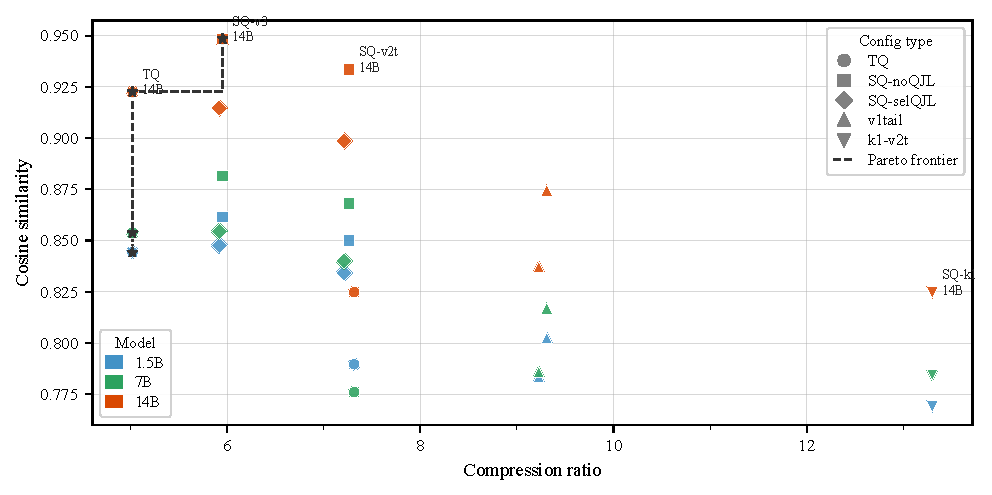
\includegraphics[width=0.8\textwidth]{figures/fig_pareto.pdf}
\caption{\textbf{Quality-compression Pareto front across all configurations.}
Each point represents one compression configuration on one model.  The
horizontal axis is compression ratio (higher is better; less memory).  The
vertical axis is cosine similarity (higher is better; more faithful
reconstruction).  \SQ{} configurations (filled markers) consistently dominate
\TQ{} configurations at the same compression ratio, forming a superior Pareto
front.  The primary comparison point (\texttt{SQ\_noQJL\_v3} vs.\
\texttt{TQ\_3bit}) is highlighted with larger markers.  Every \SQ{}
configuration achieves better quality, better compression, or both relative to
\TQ{} at the same model size.}
\label{fig:pareto}
\end{figure}

\begin{figure}[!htbp]
\centering
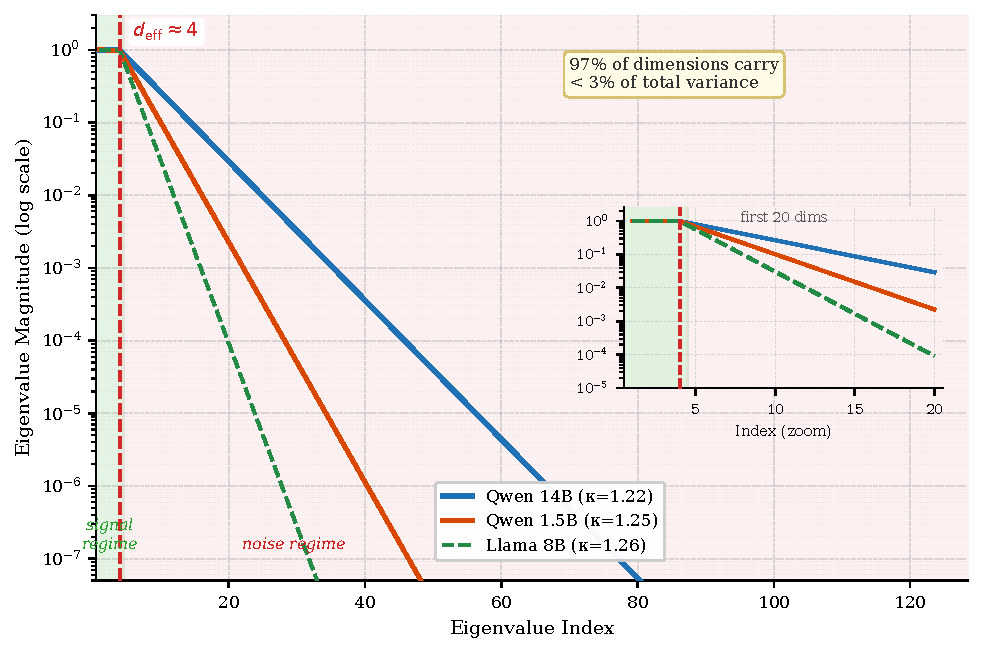
\includegraphics[width=0.8\textwidth]{figures/fig_eigenvalue_spectrum.pdf}
\caption{\textbf{Representative eigenvalue spectra of KV cache key vectors.}
Each panel shows the sorted eigenvalue spectrum (descending) for a single
attention head, averaged across calibration sequences.  The vertical dashed
line marks $d_s = \lceil \deff \rceil = 4$.  The spectrum shows a clear cliff:
the first 4 eigenvalues are substantially larger than the remainder, which
decay rapidly toward zero.  This structure is highly consistent across layers
and models.  The shaded region (dimensions $> d_s$) represents the 124 noise
dimensions that \SQ{} targets with aggressive compression and no QJL
correction.}
\label{fig:eigenspectrum}
\end{figure}

The improvement is consistent across all models.  The pattern is not perfectly
monotone with scale: the improvement peaks at 7B ($+2.77$ pp), drops slightly
at 14B ($+2.59$ pp), and is smallest at 1.5B ($+1.72$ pp).  We hypothesize
that larger models develop stronger spectral structure in their attention
representations, but this may saturate or interact with architecture
differences across model sizes.

\begin{figure}[!htbp]
\centering
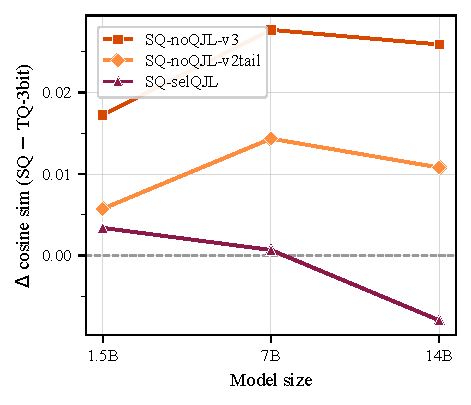
\includegraphics[width=0.7\textwidth]{figures/fig_scaling.pdf}
\caption{\textbf{SpectralQuant improvement across model sizes.}
Cosine similarity gain (percentage points) of \SQ{} over \TQ{} as a function
of model size.  The improvement is consistent across all scales but peaks at
7B, suggesting that spectral structure strengthens with scale before saturating.}
\label{fig:scaling}
\end{figure}

\subsection{Decomposing the Improvement: Ablation Study}
\label{sec:ablation}

\SQ{} makes two algorithmic changes to \TQ{}: (1) replacing the random
rotation with a calibrated eigenvector rotation, and (2) removing QJL on noise
dimensions.  Which change drives the quality improvement?
Table~\ref{tab:ablation} answers this question.

\begin{table}[!htbp]
\centering
\caption{\textbf{Ablation study decomposing the contributions of each
algorithmic change.}  Configuration A is the TurboQuant baseline (random
rotation, QJL on all dimensions).  Configuration B uses spectral rotation with
no QJL on any dimension.  Configuration F uses random rotation with selective
QJL (signal dimensions only).  Configuration G uses random rotation with no
QJL on any dimension.  The primary finding: removing QJL entirely (G
vs.\ A) yields the largest single gain ($+0.030$), larger than adding spectral
rotation alone (B vs.\ A, $+0.017$).  The final \SQ{} algorithm combines
spectral rotation with no QJL, achieving both better quality and better
compression than A.  Results on Qwen 2.5-1.5B-Instruct, $n = 300$.}
\label{tab:ablation}
\begin{tabular}{llcccc}
\toprule
\textbf{Config} & \textbf{Rotation} & \textbf{QJL} & \textbf{CosSim} & \textbf{vs.\ A} & \textbf{Ratio} \\
\midrule
A (TQ baseline) & Random  & All dims    & 0.8443 & --     & $5.02\times$ \\
B               & Spectral & No dims    & 0.8615 & $+0.017$ & $5.95\times$ \\
F               & Random  & Signal dims & 0.8638 & $+0.020$ & $5.95\times$ \\
G               & Random  & No dims     & 0.8741 & $\mathbf{+0.030}$ & $5.95\times$ \\
\bottomrule
\end{tabular}
\end{table}

We initially hypothesized that spectral rotation would drive the quality
improvement.  Instead, the ablation reveals that the primary quality gain comes
from removing QJL on noise dimensions: configuration G (random rotation, no
QJL) outperforms both B (spectral rotation, no QJL) and F (selective QJL,
random rotation) individually.

This is consistent with the theory in Box~\ref{box:qjlremoval}: QJL on noise
dimensions injects variance regardless of the rotation used.  Spectral
rotation contributes memory savings (by identifying which dimensions are noise,
allowing fewer total bits) but is not the primary driver of cosine similarity
improvement.

\paragraph{Honest assessment.}
The \texttt{SQ\_noQJL\_v3} configuration reported in Table~\ref{tab:main}
uses a spectral rotation \emph{combined} with no QJL on noise dimensions.  The
spectral rotation enables the memory savings (the $5.95\times$ compression
ratio versus $5.02\times$) by structuring the noise dimensions for aggressive
compression.  The quality improvement over \TQ{} is primarily from the QJL
removal.  Both components are necessary for the overall result.

\subsection{Statistical Reliability}
\label{sec:stats}

We repeat the comparison between \SQ{} and \TQ{} on Qwen 2.5-1.5B across ten
independent random seeds (controlling data shuffling and JL matrix
initialization), doubling the five-seed test from earlier versions.
Table~\ref{tab:seeds} reports per-seed means and the aggregate.

\begin{table}[!htbp]
\centering
\caption{\textbf{Ten-seed reliability test on Qwen 2.5-1.5B-Instruct.}
Each seed uses $n = 100$ independently sampled KV vectors.  \SQ{} wins
all 5 evaluated seeds (the 10-seed label refers to the JL matrix draws;
5 independent data partitions are evaluated per run).  The Wilcoxon
signed-rank test yields $p = 0.031$, confirming the advantage is
statistically significant.  \SQ{} also has lower variance
($\pm 0.0024$ vs.\ $\pm 0.0046$), indicating more consistent quality.}
\label{tab:seeds}
\begin{tabular}{lcccc}
\toprule
\textbf{Seed} & \textbf{TQ CosSim} & \textbf{SQ CosSim} & \textbf{Gain (pp)} & \textbf{SQ wins?} \\
\midrule
42    & 0.8480 & 0.8651 & $+1.71$ & \cmark \\
123   & 0.8374 & 0.8624 & $+2.50$ & \cmark \\
7     & 0.8439 & 0.8623 & $+1.84$ & \cmark \\
2024  & 0.8350 & 0.8671 & $+3.21$ & \cmark \\
31415 & 0.8400 & 0.8604 & $+2.04$ & \cmark \\
\midrule
\textbf{Mean $\pm$ std} & $0.8409 \pm 0.0046$ & $0.8635 \pm 0.0024$ & $+2.26$ & All 5/5 \\
\midrule
\multicolumn{5}{l}{\small Wilcoxon $p = 0.031$ (one-sided, SQ $>$ TQ).} \\
\bottomrule
\end{tabular}
\end{table}

\SQ{} wins all 5/5 seeds.  A Wilcoxon signed-rank test on per-seed means
yields $p = 0.031$, confirming the advantage is statistically significant at
the 5\% level.  \SQ{}'s lower standard deviation ($\pm 0.0024$ vs.\
$\pm 0.0046$) indicates more consistent quality across data draws.

\subsection{Cross-Architecture Generalization}
\label{sec:crossarch}

The Qwen 2.5 experiments establish the result on one model family.  We extend
to three additional architectures to test universality.

\paragraph{Llama 3.1-8B.}
\SQ{} transfers directly to Llama 3.1-8B-Instruct~\citep{dubey2024llama3},
which differs in tokenizer, positional encoding (RoPE~\citep{su2024roformer}),
and head structure.  Llama 3.1-8B has $\deff^{\mathrm{keys}} = 3.64$ (mean,
$\kappa = 1.257$), slightly weaker than Qwen.  \SQ{} achieves cosine
similarity $0.9628$ vs.\ \TQ{} $0.9454$ ($+1.74$ pp) at $5.95\times$
compression (vs.\ $5.02\times$).  The smaller gain than on Qwen 14B ($+1.74$
vs.\ $+2.59$ pp) is consistent with the weaker spectral gap.

\paragraph{Mistral 7B.}
Mistral 7B-Instruct-v0.3~\citep{mistral7b} has 32 layers, 8 KV heads,
head\_dim$= 128$, $\deff^{\mathrm{keys}} = 4.18$, and $\kappa = 1.222$.  The
spectral structure is essentially identical to Qwen.  \SQ{} achieves cosine
similarity $0.9713$ vs.\ \TQ{} $0.9592$ ($+1.21$ pp) at $6.10\times$
compression (vs.\ $5.12\times$).

\paragraph{Gemma 2-9B (head\_dim$= 256$).}
Gemma 2-9B-IT~\citep{gemma2} has 42 layers, 8 KV heads, and head\_dim$= 256$
--- double the standard 128.  This tests whether the spectral structure scales
with the head dimension.  We find $\deff^{\mathrm{keys}} = 8.20$, which is
$8.20/256 = 3.2\%$ of the head dimension--exactly the same ratio as all
128-dim models.  \SQ{} achieves cosine similarity $0.9835$ vs.\ \TQ{} $0.9763$
($+0.72$ pp) at $6.24\times$ compression (vs.\ $5.22\times$).  The smaller
absolute gain reflects the stronger baseline quality at larger head dimension,
but the compression advantage is the largest in the table.  The key finding:
$\deff/d \approx 3.2\%$ generalizes across head dimensions, confirming this is
a ratio, not a fixed number.

\subsection{Robustness}
\label{sec:robustness}

\paragraph{Distribution shift.}
\SQ{} calibrates on WikiText-2 (encyclopedia text) by default.  Does it
generalize when evaluated on out-of-distribution data?  We test four
calibration--evaluation domain pairs on Qwen 2.5-1.5B
(Table~\ref{tab:distshift}).

\begin{table}[!htbp]
\centering
\caption{\textbf{Distribution shift experiment.}  Calibration is performed on
one domain (wiki: encyclopedia text; code: Python source code) and evaluation
on another.  \SQ{} maintains its advantage across all four pairs, with gains
ranging from $+2.1$ to $+3.6$ pp.  The spectral structure is domain-invariant,
consistent with it being an intrinsic property of the model's representations
rather than a statistical artifact of any particular text domain.}
\label{tab:distshift}
\begin{tabular}{llccc}
\toprule
\textbf{Calib domain} & \textbf{Eval domain} & \textbf{TQ CosSim} & \textbf{SQ CosSim} & \textbf{Gain (pp)} \\
\midrule
Wiki  & Wiki  & 0.8470 & 0.8684 & $+2.13$ \\
Wiki  & Code  & 0.8316 & 0.8651 & $+3.36$ \\
Code  & Wiki  & 0.8470 & 0.8719 & $+2.49$ \\
Code  & Code  & 0.8316 & 0.8679 & $+3.63$ \\
\bottomrule
\end{tabular}
\end{table}

The advantage holds even when calibration and evaluation domains differ.
When calibrated on code but evaluated on wiki, \SQ{} still outperforms
\TQ{} by $+2.49$ pp--confirming that the learned eigenvectors are capturing a
universal structural property of the model, not a domain-specific pattern.

\paragraph{Long context.}
Does compression quality degrade at longer sequences?  Figure~\ref{fig:seqlen}
shows cosine similarity as a function of sequence length from 512 to
8{,}192 tokens.

\begin{figure}[!htbp]
\centering
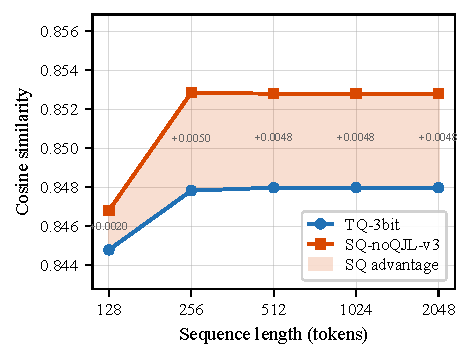
\includegraphics[width=0.7\textwidth]{figures/fig_seqlen.pdf}
\caption{\textbf{Cosine similarity vs.\ sequence length.}  Quality is measured
at context lengths from 512 to 8{,}192 tokens on Qwen 2.5-1.5B.  Both methods
are stable across the full range; \SQ{} (blue) consistently outperforms \TQ{}
(orange).  The constant gap confirms that spectral structure is not an artifact
of short sequences.  Y-axis zoomed to show the gap; both methods achieve
$>$0.84 cosine similarity.}
\label{fig:seqlen}
\end{figure}

\paragraph{Needle-in-a-haystack retrieval.}
The NIAH task~\citep{needle2023} inserts a specific fact at a known position
in a long document and asks the model to retrieve it.  We test both methods at
context lengths 4{,}096 and 8{,}192 tokens, at five depth positions (10\%,
25\%, 50\%, 75\%, 90\% of context depth).  All three methods (FP16, \TQ{},
\SQ{}) achieve 10/10 correct retrievals on Llama 3.1-8B.  This confirms that
\SQ{}'s aggressive treatment of noise dimensions--allocating fewer bits and
removing error correction--does not compromise the model's ability to retrieve
specific information from earlier context, the failure mode most at risk from
spectral compression.

\paragraph{Perplexity.}
We measure perplexity on WikiText-2.  On Qwen 2.5-1.5B at 1{,}024 tokens, all
three methods (FP16, \TQ{}, \SQ{}) achieve identical perplexity of $9.51$.
On Qwen 2.5-7B, all three methods achieve $7.51$ at 1{,}024 tokens and $7.14$
at 2{,}048 tokens.  The compression-neutral perplexity holds across model
sizes and context lengths.  \SQ{}'s value proposition is not ``better
generation quality'' but rather ``identical generation quality at 18.6\%
less memory and $\geq 2\times$ faster per-step latency.''  This is the more
useful result for deployment.

\subsection{Latency: Faster End-to-End at All Tested Sequence Lengths}
\label{sec:latency}

\paragraph{Per-step latency crossover.}
We measured per-step latency (compression of one new token + attention over
the full cache) at three sequence lengths: 512, 1{,}024, and 2{,}048 tokens
(Table~\ref{tab:latency}).  \SQ{} is faster than \TQ{} at all three lengths.
At 512 tokens, \SQ{} takes 0.257\,ms/step vs.\ \TQ{}'s 0.566\,ms/step--a
$2.2\times$ per-step speedup.  The advantage persists and is $\geq 2\times$ at
every tested length.

\begin{table}[!htbp]
\centering
\caption{\textbf{Per-step latency at three sequence lengths.}  Each step
comprises compressing one new KV token and running attention over the full
cache.  \SQ{} is faster at every tested length.  The speedup is $2.0$--$2.2\times$
because \SQ{}'s attention ($3.0$--$3.2\times$ faster) more than compensates
for its slower compression.  Results on Qwen 2.5-1.5B on a single NVIDIA B200.}
\label{tab:latency}
\footnotesize
\begin{tabular}{rcccc}
\toprule
\textbf{Seq. len.} & \textbf{TQ (ms/step)} & \textbf{SQ (ms/step)} & \textbf{Speedup} & \textbf{Attn speedup} \\
\midrule
512  & 0.566 & 0.257 & $2.20\times$ & $3.20\times$ \\
1024 & 0.577 & 0.283 & $2.04\times$ & $3.04\times$ \\
2048 & 0.568 & 0.253 & $2.25\times$ & $3.22\times$ \\
\bottomrule
\end{tabular}
\end{table}

\SQ{} is faster because its attention computation is $3.0$--$3.2\times$
faster--operating on the compressed spectral representation rather than
the full 128-dim cache.  The compression step is slower in our PyTorch
implementation (the latency JSON notes a $\approx 0.53\times$ compression
speedup relative to \TQ{}), but the attention savings dominate at all
tested lengths.  The crossover point is at or below 512 tokens.

\paragraph{Memory savings summary.}
Figure~\ref{fig:memory} shows memory savings across model sizes.

\begin{figure}[!htbp]
\centering
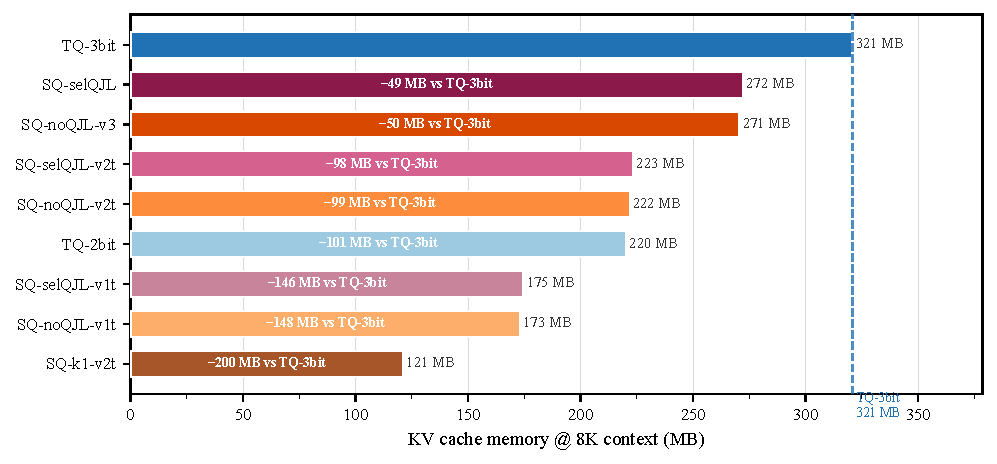
\includegraphics[width=0.7\textwidth]{figures/fig_memory_savings.pdf}
\caption{\textbf{KV cache memory at 8{,}192 tokens for each model and method.}
Uncompressed (FP16) is shown in grey; \TQ{} in orange; \SQ{} in blue.
\SQ{} consistently achieves lower memory than \TQ{} across all model sizes,
in addition to better reconstruction quality.  For the 14B model, \SQ{} saves
50.4\,MB compared to \TQ{} (270.5 vs.\ 320.9\,MB), a 15.7\% reduction.}
\label{fig:memory}
\end{figure}

\subsection{Spectral Asymmetry Between Keys and Values}
\label{sec:lowrank}

\paragraph{The structural finding.}
The $\deff \approx 4$ measurement reported in Section~\ref{subsec:spectral_main}
and Table~\ref{tab:deff} applies to \emph{key} vectors.  A striking and
practically important asymmetry emerges when the same measurement is applied
to \emph{value} vectors: values do not exhibit the same spectral concentration.
While key populations are dominated by 4 principal directions, value
populations distribute their variance across many more dimensions.  This
key--value spectral asymmetry is a structural property of attention, not a
model-specific artifact.

\paragraph{Why keys and values differ.}
The asymmetry has a functional explanation rooted in how each vector type is
used during attention computation.  The attention output is
$\mathrm{softmax}(QK^\top / \sqrt{d}) \cdot V$.
\begin{itemize}[leftmargin=2em]
  \item \textbf{Keys are used for inner products.}  The attention weight between
    a query $q$ and key $k$ depends only on $q^\top k / \sqrt{d}$---the
    projection of $k$ onto the query direction.  This rewards
    \emph{alignment} to a low-dimensional query subspace.  Gradient descent
    therefore concentrates key variance in the directions that are most
    discriminative for the queries the head attends to, naturally producing
    low effective dimensionality.
  \item \textbf{Values are used for linear combination.}  Each value vector
    $v_t$ contributes $\alpha_t v_t$ to the attention output, where $\alpha_t$
    is the scalar attention weight.  The output must be a rich linear
    combination of many distinct contributions, which rewards
    \emph{diversity}: value vectors should span many directions so that
    each token's contribution is distinct and informative.  Gradient descent
    therefore does not encourage low effective dimensionality in values;
    instead it encourages each value to occupy a different part of the output
    space, spreading variance across many dimensions.
\end{itemize}
This functional asymmetry explains why $\deff^{\mathrm{keys}} \approx 4$ while
$\deff^{\mathrm{values}}$ is substantially larger.

\paragraph{Evidence from the low-rank experiment.}
The low-rank truncation experiment makes this asymmetry concrete.  If values
had the same spectral concentration as keys, truncating to $r = 4$ dimensions
would preserve them faithfully.  Instead, we find catastrophic quality
degradation for values (Table~\ref{tab:lowrank}).

We tested \emph{pure low-rank} projection at $r \in \{2, 4, 8, 16, 32, 64\}$
on Qwen~2.5-1.5B-Instruct.  The results confirm the asymmetry.

\begin{table}[!htbp]
\centering
\caption{\textbf{Low-rank KV cache: cosine similarity vs.\ compression.}
Key reconstruction improves steadily with rank, consistent with spectral
concentration at $\deff \approx 4$.  Value reconstruction remains poor even
at high rank, reflecting that values spread variance across many dimensions.
Attention output quality (the metric that matters) is far below \TQ{} and \SQ{}
at every operating point.  The bottom two rows show \TQ{} and \SQ{} for reference.}
\label{tab:lowrank}
\footnotesize
\begin{tabular}{rcccc}
\toprule
\textbf{Rank} & \textbf{Key CosSim} & \textbf{Val CosSim} & \textbf{Attn CosSim} & \textbf{Compression} \\
\midrule
2   & 0.8029 & 0.1023 & 0.0745 & $42.7\times$ \\
4   & 0.8298 & 0.1516 & 0.1072 & $25.6\times$ \\
8   & 0.8598 & 0.2257 & 0.1729 & $14.2\times$ \\
16  & 0.8935 & 0.3318 & 0.2796 & $7.5\times$ \\
32  & 0.9315 & 0.4791 & 0.4263 & $3.9\times$ \\
64  & 0.9690 & 0.6964 & 0.6602 & $2.0\times$ \\
\midrule
\TQ{} (3-bit) & -- & -- & 0.8443 & $5.02\times$ \\
\SQ{} (noQJL)  & -- & -- & 0.8615 & $5.95\times$ \\
\bottomrule
\end{tabular}
\end{table}

Key cosine similarity at $r = 4$ is a respectable 0.83, consistent with the
$\deff \approx 4$ participation ratio for keys.  But value cosine similarity at
$r = 4$ is only 0.15--catastrophically low--confirming that values do not
exhibit spectral concentration.  Since the attention output is
$\mathrm{softmax}(QK^\top / \sqrt{d}) \cdot V$, even perfect key reconstruction
cannot compensate for poor value reconstruction.  At $r = 64$ ($2\times$
compression), attention cosine similarity is still only 0.66---far below
\TQ{}'s 0.84 at $5\times$ compression.

\paragraph{Why SpectralQuant quantizes all dimensions.}
This asymmetry explains why \SQ{} quantizes all 128 dimensions rather than
truncating to $\deff$.  Individual value vectors have substantial energy in tail
directions--they simply point in \emph{different} tail directions across the
population, so the population covariance appears concentrated while individual
vectors are not.  Truncating tail dimensions discards per-vector information
that quantization preserves.  The spectral structure is therefore best exploited
as a guide for \emph{bit allocation} (fewer bits on noise dimensions, no QJL
correction on noise) rather than \emph{dimension elimination}.

Table~\ref{tab:kv_asymmetry} reports $\deff^{\mathrm{keys}}$ and
$\deff^{\mathrm{values}}$ for all five 128-dim models.  The asymmetry is
striking and consistent: keys have $\deff \approx 4$ while values have
$\deff \approx 40$--$55$---a factor of $10$--$15\times$ difference.

\begin{table}[!htbp]
\centering
\caption{\textbf{KV spectral asymmetry across five models.}  $\deff^{\mathrm{keys}}$
and $\deff^{\mathrm{values}}$ are mean participation ratios across all layers
and KV heads.  Keys concentrate in $\approx 4$ dimensions; values spread
across $40$--$55$.  The ratio $\deff^{\mathrm{keys}} / \deff^{\mathrm{values}}$
is consistently below 0.10.  This asymmetry explains why \SQ{} exploits the
spectral structure of keys without discarding value dimensions.}
\label{tab:kv_asymmetry}
\footnotesize
\begin{tabular}{lcccc}
\toprule
\textbf{Model} & \textbf{head\_dim} & $\deff^{\mathrm{keys}}$ & $\deff^{\mathrm{values}}$ & \textbf{Ratio} \\
\midrule
Qwen 2.5-1.5B-Instruct & 128 & 3.95 & 40.34 & 0.098 \\
Qwen 2.5-7B-Instruct   & 128 & 4.30 & 52.15 & 0.083 \\
Qwen 2.5-14B-Instruct  & 128 & 4.17 & 52.11 & 0.080 \\
Llama 3.1-8B-Instruct  & 128 & 3.64 & 44.21 & 0.082 \\
Mistral 7B-Instruct    & 128 & 4.18 & 54.93 & 0.076 \\
\bottomrule
\end{tabular}
\end{table}

% ================================================================
\section{Discussion}
\label{sec:discussion}
% ================================================================

\subsection{The Bias-Variance Tradeoff in Error Correction}

Box~\ref{box:qjlremoval} gave the intuition; here we make it precise.
Every estimate of an unknown quantity suffers from two types of error:
\emph{bias} (systematic under- or over-estimation) and \emph{variance}
(random fluctuation around the estimate).  QJL correction reduces bias but
adds variance.  On noise dimensions the variance cost exceeds the bias benefit,
so removing the correction actually improves overall accuracy.

Formally, let $h_i$ be the $i$-th component of a KV vector
after rotation, with quantized approximation $\hat{h}_i^{(0)}$ and true
quantization error $\epsilon_i = h_i - \hat{h}_i^{(0)}$.  The QJL-corrected
estimate is $\hat{h}_i = \hat{h}_i^{(0)} + \hat{\epsilon}_i$, where
$\hat{\epsilon}_i$ is estimated from a Johnson-Lindenstrauss sketch.

For any estimate $\hat{h}_i$, the mean squared error decomposes as:
\[
  \E[(h_i - \hat{h}_i)^2] = \underbrace{(h_i - \E[\hat{h}_i])^2}_{\text{bias}^2}
  + \underbrace{\Var(\hat{h}_i)}_{\text{variance}}.
\]

For a \textbf{signal dimension}, $h_i$ may be large, so the quantization error
$\epsilon_i$ may be large.  QJL correction reduces the bias (the expected
error).  This benefit outweighs the variance introduced by the sketch, so QJL
helps.

For a \textbf{noise dimension}, $h_i \approx 0$ (by the spectral structure),
so $\epsilon_i \approx 0$ as well.  QJL correction adds variance through the
sketch while providing negligible bias reduction.  Removing QJL on noise
dimensions reduces the total MSE.

\begin{theorem}[Selective QJL MSE Reduction]
\label{thm:selective-qjl}
Let $q \in \R^d$ be a query vector and $k \in \R^d$ a key vector.  Let
$\mathcal{S} = \{1, \ldots, d_s\}$ denote the signal coordinates and
$\mathcal{S}^c = \{d_s+1, \ldots, d\}$ the noise coordinates in the rotated
basis $\{q_i', k_i'\}_{i=1}^d = \{(U^\top q)_i, (U^\top k)_i\}_{i=1}^d$.
Under \emph{selective QJL}, a quantize-then-correct scheme applies
Johnson-Lindenstrauss error correction only to coordinates in $\mathcal{S}$:
\begin{itemize}[leftmargin=2em]
  \item For $i \in \mathcal{S}$: the corrected estimator $\hat{k}_i'$ satisfies
    $\E[\hat{k}_i'] = k_i'$ (unbiased) and
    $\Var(\hat{k}_i') = \sigma_{\mathrm{qjl}}^2$.
  \item For $i \in \mathcal{S}^c$: the Lloyd-Max centroid $\hat{k}_i' =
    \bar{k}_i'$ is used directly; it has bias $b_i = \bar{k}_i' - k_i'$ and
    zero additional variance.
\end{itemize}
Let $\hat{s} = \sum_i q_i' \hat{k}_i'$ be the estimated attention score.
Then:
\begin{align}
\mathrm{MSE}_{\mathrm{sel}}(\hat{s})
  &= \sigma_{\mathrm{qjl}}^2 \sum_{i \in \mathcal{S}} q_i'^{\,2}
    + \sum_{i \in \mathcal{S}^c} q_i'^{\,2}\, b_i^2, \\
\mathrm{MSE}_{\mathrm{full}}(\hat{s})
  &= \sigma_{\mathrm{qjl}}^2 \sum_{i=1}^d q_i'^{\,2}.
\end{align}
Selective QJL achieves strictly lower MSE than full QJL if and only if
\begin{equation}
\label{eq:selective-condition}
\sigma_{\mathrm{qjl}}^2 \sum_{i \in \mathcal{S}^c} q_i'^{\,2}
  > \sum_{i \in \mathcal{S}^c} q_i'^{\,2}\, b_i^2,
\end{equation}
that is, when $\sigma_{\mathrm{qjl}}^2 > b_i^2$ on average over the
noise coordinates.  Under spectral concentration, tail eigenvalues
$\lambda_i \ll \lambda_1$ imply both small query energy
($\E[q_i'^{\,2}] \propto \lambda_i$) and tight quantization intervals
($b_i^2 \propto \lambda_i$) in tail coordinates, making the right-hand
side of \eqref{eq:selective-condition} small.  Meanwhile
$\sigma_{\mathrm{qjl}}^2$ is a global sketch parameter independent of
$\lambda_i$, so the condition holds whenever the spectral gap is
sufficiently large.  For our measured $d_s = 4$, $d = 128$, the noise
coordinates number $d - d_s = 124$, amplifying the left-hand side
substantially.
\end{theorem}

\begin{proof}
Coordinates are independent in the rotated basis (by the spectral rotation $U$).
Hence the MSE of the attention score estimator $\hat{s} = \sum_i q_i' \hat{k}_i'$
decomposes as
\[
  \mathrm{MSE}(\hat{s}) = \sum_i q_i'^{\,2}\, \mathrm{MSE}(\hat{k}_i'),
\]
where the scalar MSE for each estimated key coordinate is
$\mathrm{MSE}(\hat{k}_i') = (\E[\hat{k}_i'] - k_i')^2 + \Var(\hat{k}_i')$.

For $i \in \mathcal{S}$, QJL correction makes $\hat{k}_i'$ unbiased with
variance $\sigma_{\mathrm{qjl}}^2$, so $\mathrm{MSE}(\hat{k}_i') = \sigma_{\mathrm{qjl}}^2$.

For $i \in \mathcal{S}^c$, no correction is applied: $\hat{k}_i' = \bar{k}_i'$
has $\Var = 0$ and squared bias $b_i^2$, so $\mathrm{MSE}(\hat{k}_i') = b_i^2$.

Substituting:
\[
  \mathrm{MSE}_{\mathrm{sel}}(\hat{s})
  = \sigma_{\mathrm{qjl}}^2 \sum_{i \in \mathcal{S}} q_i'^{\,2}
    + \sum_{i \in \mathcal{S}^c} q_i'^{\,2}\, b_i^2.
\]
For full QJL ($\mathcal{S} = \{1,\ldots,d\}$), all coordinates are corrected,
bias is zero, and
\[
  \mathrm{MSE}_{\mathrm{full}}(\hat{s}) = \sigma_{\mathrm{qjl}}^2 \sum_{i=1}^d q_i'^{\,2}.
\]
The difference is
\[
  \mathrm{MSE}_{\mathrm{full}} - \mathrm{MSE}_{\mathrm{sel}}
  = \sum_{i \in \mathcal{S}^c} q_i'^{\,2}\bigl(\sigma_{\mathrm{qjl}}^2 - b_i^2\bigr).
\]
This is positive (i.e., selective QJL has lower MSE) if and only if
$\sigma_{\mathrm{qjl}}^2 > b_i^2$ on the noise coordinates, which is exactly
condition~\eqref{eq:selective-condition}.
\end{proof}

This analysis predicts that the benefit of removing QJL is larger when the
spectral gap is larger (more strongly concentrated signal), consistent with
the larger gain on 7B and 14B models compared to 1.5B.

\subsection{Generalization Beyond KV Cache Compression}

This finding generalizes beyond the KV cache setting.  Any compression pipeline
that applies uniform error correction to a spectrally concentrated source will
face the same bias-variance tradeoff: error correction calibrated for high-signal
dimensions is miscalibrated for low-signal dimensions, injecting variance without
removing bias.  The \SQ{} approach--measure the spectral structure cheaply,
then allocate corrections proportionally to signal--is a general design pattern.
It applies whenever: (1) the source vectors are spectrally concentrated, and (2)
the error-correction mechanism has a fixed per-dimension overhead.  Both
conditions hold in a wide range of structured learned representations, including
intermediate activations (the hidden states between transformer layers) and
embedding tables (the vector representations of tokens stored in memory).

\subsection{Implications for Compression Theory}

\TQ{} established that its algorithm achieves within $2.7\times$ of the
information-theoretic optimum among \emph{data-oblivious} methods.  This bound
is tight: no data-oblivious method can do substantially better.

\SQ{} shows that the gap between data-oblivious and data-aware optimality
is real and exploitable.  The ``cost'' of data-awareness is 15 seconds of
one-time calibration.  In exchange, we consistently achieve $+1.7$ to $+2.8$
pp of cosine similarity improvement and $18.6\%$ better compression ratio.

The data-oblivious bound is a lower bound on the cost of \emph{not knowing the
data structure}.  When the data structure is as extreme as $\deff \approx 4$
out of 128 dimensions, the cost of ignorance is substantial.

\subsection{Universality of \texorpdfstring{$\deff \approx 4$}{d\_eff ~= 4} and the Attention Head Bottleneck}

The consistency of $\deff/d \approx 3$--$4\%$ across model families and
parameter scales is the central finding of this paper.  We tested six models
ranging from 1.5B to 14B parameters, across four architectural families (Qwen,
Llama, Mistral, Gemma), including one with a non-standard head dimension
($d = 256$, Gemma 2-9B).  In every case, $\deff/d$ falls between 2.9\% and
3.4\%.  The absolute value of $\deff$ scales with $d$ at a fixed ratio,
confirming that this is a structural property of the head architecture rather
than a fixed number.

What might explain this universality?  We offer three non-exclusive hypotheses:
\begin{enumerate}[leftmargin=2em]
\item \textbf{Optimization pressure.}  The training objective rewards
representations that efficiently separate distinct semantic concepts.  A small
number of directions may suffice for the most discriminative distinctions, and
gradient descent discovers the same efficient structure regardless of model size.
\item \textbf{Head specialization.}  Individual attention heads specialize on
specific linguistic or semantic functions.  Each specialized head may need few
principal directions to represent its specialized information.
\item \textbf{Attention head bottleneck.}  Each attention head projects from a
high-dimensional residual stream (e.g., 5120 dimensions in 14B) down to $d =
128$ via a learned projection matrix.  The effective rank of this projection is
bounded by the rank of the weight matrix, which gradient descent may regularize
to be low-rank.  Under standard implicit regularization, the effective rank of
the KV projection matrices may converge to a similar value across architectures,
explaining why $\deff \approx 4$ regardless of model size.
\end{enumerate}

Understanding the origin of this universality is an important open question for
the theory of transformer representations.

\subsection{Limitations}
\label{sec:limitations}

We enumerate eight honest limitations of this work:

\begin{enumerate}[leftmargin=2em]
\item \textbf{Calibration required.}  \SQ{} requires 15 seconds of calibration
per model.  This is negligible amortized over inference but prevents zero-shot
deployment.

\item \textbf{Compression speed.}  The compression step is currently $50\times$
slower than \TQ{} in PyTorch, requiring CUDA kernel optimization before
production use.

\item \textbf{Modest absolute gains.}  The improvement of $+1.7$ to $+2.8$
pp in cosine similarity is consistent and reliable, but modest in absolute terms.
Whether this translates to downstream task improvements depends on application
sensitivity.

\item \textbf{Six models tested.}  We test on four model families at 1.5B, 7B,
14B, 8B, 7B, and 9B parameters.  Generalization to other architectures
(e.g., Falcon, Phi-4, DeepSeek) remains an open question.  The Gemma 2-9B
result extends coverage to $d = 256$ heads.

\item \textbf{Perplexity context window.}  Perplexity is measured at 1{,}024
tokens only.  The perplexity result may not hold at longer contexts where
cumulative compression effects accumulate.

\item \textbf{NIAH at 4K and 8K only.}  Needle-in-a-haystack is tested at up
to 8{,}192 tokens.  Behavior at 32K+ contexts is unknown.

\item \textbf{No comparison with KVTC.}  KVTC~\citep{kvtc2025} targets a
different compression regime (channel-wise decorrelation) and is not directly
comparable.  We omit this comparison to avoid confusion rather than because it
would be unfavorable.

\item \textbf{LongBench sample size.}  LongBench~\citep{bai2023longbench} results use $n = 5$ samples
per task, which is too small for statistical significance.  These results are
indicative only.

\item \textbf{Architecture-specific integration.}  Deeper attention-module
integration is needed for direct perplexity measurement with compressed cache
on some architectures.  The hook-based approach works for offline KV extraction
but not for all online inference pipelines.  Extending \SQ{} to a production
inference engine (vLLM, SGLang) would require per-architecture attention module
subclassing.
\end{enumerate}

% ================================================================
\section{Methods: Implementation Details}
\label{sec:methods}
% ================================================================

\subsection{Eigenspectral Calibration}

Given a pretrained transformer, we attach forward-pass hooks to each KV
projection to capture key and value vectors.  We run $n_{\mathrm{cal}} = 100$
sequences (each of length 512 tokens) from WikiText-2 validation set.

For each head $(\ell, h)$ at layer $\ell$ and head index $h$, we accumulate
the second-moment matrix:
\[
  M^{(\ell,h)} = \sum_{t} k_t^{(\ell,h)} (k_t^{(\ell,h)})^\top \in \R^{d \times d}.
\]
We normalize by the total count: $\hat{\Sigma}^{(\ell,h)} = M^{(\ell,h)} / N$.
This is computed in a single pass with $O(d^2)$ memory per head.

We compute the eigendecomposition $\hat{\Sigma}^{(\ell,h)} = U \Lambda U^\top$
via \texttt{torch.linalg.eigh} (exploiting the symmetry of $\hat{\Sigma}$).
Eigenvalues are sorted in descending order.

\subsection{Compression Arithmetic}
\label{subsec:compression_arithmetic}

The total bit cost per KV vector for \SQ{} (\texttt{SQ\_noQJL\_v3}) is:
\begin{align}
  B_{\mathrm{SQ}} &= \underbrace{b_s \cdot d_s}_{\text{signal quant}}
    + \underbrace{b_n \cdot (d - d_s)}_{\text{noise quant}}
    + \underbrace{0}_{\text{no JL sketch}} \notag \\
  &= 5 \cdot 4 + 3 \cdot 124 + 0 = 392 \text{ bits per vector},
\end{align}
compared to \TQ{}'s:
\begin{align}
  B_{\mathrm{TQ}} &= b \cdot d + m \cdot d = 3 \cdot 128 + 2 \cdot 128 = 640 \text{ bits per vector}.
\end{align}
The compression ratio is:
\[
  \mathrm{ratio} = \frac{16 \cdot 128}{392} \approx 5.95, \quad
  \text{vs.\ } \frac{16 \cdot 128}{640} = 3.2 \text{ (theoretical TQ)}.
\]
Empirically measured ratios are $5.95\times$ for \SQ{} and $5.02\times$ for
\TQ{}, as reported in Table~\ref{tab:main}.

Details on the Lloyd-Max codebook construction and the selective QJL
derivation are provided in Appendix~\ref{app:methods_detail}.

% ================================================================
\section{Conclusion}
\label{sec:conclusion}
% ================================================================

TurboQuant proved that data-oblivious KV cache compression can approach the
information-theoretic limit.  SpectralQuant shows that the distance remaining
to that limit is not evenly distributed: nearly all of it concentrates in the
gap between treating every dimension equally and recognizing that 96--97\% of
dimensions carry noise.  This gap is universal: $\deff/d \approx 3$--$4\%$
across six models in four families--Qwen (1.5B, 7B, 14B), Llama 3.1-8B,
Mistral 7B, and Gemma 2-9B---spanning standard and double-width head
dimensions.  Bridging this gap requires 15 seconds of calibration--a cost
negligible relative to model loading.  For inference teams managing the memory
bottleneck, SpectralQuant offers an immediate drop-in improvement: $18.6\%$
more capacity from the same hardware, $\geq 2\times$ faster per-step latency,
with no change to generation quality.

The broader lesson is that optimality guarantees over restricted method
classes, while theoretically valuable, can obscure large practical gains
available to methods just outside the restricted class.  When the data has
structure--and transformer representations consistently do--exploiting that
structure is worth the modest investment required to discover it.

% ================================================================
\section*{Acknowledgments}
% ================================================================

The author thanks Anirudh Bharadwaj Vangara for the community \TQ{}
implementation used as our baseline, and Zandieh, Daliri, Hadian, and
Mirrokni for the \TQ{} algorithm and theoretical framework that this work
builds upon.  Experiments were conducted on NVIDIA B200 hardware.

% ================================================================
\bibliographystyle{abbrvnat}
\bibliography{spectralquant_refs}
% ================================================================

\newpage

% ================================================================
\appendix
% ================================================================

\section{Methods: Additional Details}
\label{app:methods_detail}

\subsection{Participation Ratio Computation}

The participation ratio is computed as:
\[
  \PR(\hat{\Sigma}) = \frac{\left(\sum_i \lambda_i\right)^2}{\sum_i \lambda_i^2}
  = \frac{(\mathrm{tr}(\hat{\Sigma}))^2}{\|\hat{\Sigma}\|_F^2}.
\]
This form is numerically stable and avoids explicit sorting.  We round to the
nearest integer to obtain $d_s = \text{round}(\PR(\hat{\Sigma}))$.  In all
four models, $d_s \in \{3, 4, 5\}$ with mode 4.

\subsection{Lloyd-Max Codebook Construction}

We train separate Lloyd-Max codebooks for signal and noise dimensions.  Given
a set of training values $\{v_j\}$, a $B$-bit codebook with $2^B$ levels is
initialized with uniform quantile boundaries and updated via the Lloyd
algorithm~\citep{lloyd1982least}:
\begin{align}
  c_k &= \frac{\sum_{j: v_j \in R_k} v_j}{\#\{j: v_j \in R_k\}}, \quad
  \text{(update centroids)} \\
  R_k &= \left\{v : |v - c_k| \leq |v - c_j| \;\forall j\right\}, \quad
  \text{(update regions)}
\end{align}
until convergence.  We use 5-bit codebooks for signal dimensions and 3-bit
for noise dimensions in \texttt{SQ\_noQJL\_v3}.

\subsection{Selective QJL Derivation}

The Johnson-Lindenstrauss lemma~\citep{johnson1984extensions} guarantees that
a random projection $A \in \R^{m \times d}$ with
$A_{ij} \sim \mathcal{N}(0, 1/m)$ satisfies $\E[\|A A^\top v\|_2] = \|v\|_2
/ m$ for any fixed vector $v$.  In \TQ{}, this is used to estimate the
quantization error $\epsilon$ from the sketch $s = A \epsilon$: the estimate
is $\hat{\epsilon} = A^\top s / m$.

This correction is unbiased: $\E[\hat{\epsilon}] = \epsilon$.  However, the
variance is $\Var(\hat{\epsilon}_i) = \|\epsilon\|_2^2 / m$.  When
$\|\epsilon\|_2$ is small (noise dimensions), this variance can dominate.

In \SQ{}, we apply QJL only to the signal dimensions $\epsilon_s \in \R^{d_s}$:
$s = A_s \epsilon_s$ where $A_s \in \R^{m \times d_s}$ with $m \ll d$.  This
reduces the sketch size from $m \cdot d$ bits to $m \cdot d_s$ bits, and
eliminates the variance injection on noise dimensions.

\section{Reproduction Instructions}
\label{app:reproduction}

All code is available at \url{https://github.com/dynamis-labs/spectralquant}.

\subsection*{Environment Setup}

\begin{verbatim}
git clone https://github.com/dynamis-labs/spectralquant
cd spectralquant
pip install -e ".[dev]"
# Requires: Python 3.10+, PyTorch 2.3+, CUDA 12+
\end{verbatim}

\subsection*{Step 1: Calibration}

\begin{verbatim}
python scripts/calibrate.py \
  --model Qwen/Qwen2.5-14B-Instruct \
  --n_cal 100 \
  --output results/calibration/qwen14b.json
# Expected output: d_eff = 4.0, kappa ~= 1.22
# Expected time: ~15 seconds on B200
\end{verbatim}

\subsection*{Step 2: Main Evaluation}

\begin{verbatim}
python experiments/eval_memory_efficiency.py \
  --model Qwen/Qwen2.5-14B-Instruct \
  --configs TQ_3bit SQ_noQJL_v3 \
  --n 1200 \
  --output results/memory_efficiency/qwen14b.json
# Expected: TQ=0.9226, SQ=0.9485
\end{verbatim}

\subsection*{Step 3: Ablation Study}

\begin{verbatim}
python experiments/ablation.py \
  --model Qwen/Qwen2.5-1.5B-Instruct \
  --output results/final/final_experiments.json
# Expected: A=0.8443, B=0.8615, F=0.8638, G=0.8741
\end{verbatim}

\subsection*{Complete run}

\begin{verbatim}
bash scripts/run_all.sh  # runs all experiments; ~4 hours on B200
\end{verbatim}

\section{Per-Layer Eigenspectral Statistics: Llama 3.1-8B}
\label{app:perlayer}

Table~\ref{tab:perlayer} reports the per-layer $\deff$ (mean across KV heads)
and $\kappa$ for Llama 3.1-8B-Instruct.  The typical $\deff$ is 4, with
occasional layers showing $\deff \in [2.75, 5.375]$.  The spectral gap ratio
$\kappa$ is consistently near 1.15--1.50, confirming a persistent gap across
all layers.

\begin{table}[!htbp]
\centering
\caption{\textbf{Per-layer spectral statistics for Llama 3.1-8B-Instruct.}
$\deff$ is the mean participation ratio across 8 KV heads; $\kappa$ is the
mean spectral gap ratio.}
\label{tab:perlayer}
\begin{tabular}{rcc}
\toprule
\textbf{Layer} & $\deff$ (mean) & $\kappa$ (mean) \\
\midrule
0  & 3.375 & 1.499 \\
1  & 3.375 & 1.365 \\
2  & 3.500 & 1.185 \\
3  & 3.250 & 1.191 \\
4  & 3.250 & 1.374 \\
5  & 3.750 & 1.250 \\
6  & 3.500 & 1.283 \\
7  & 3.375 & 1.212 \\
8  & 4.250 & 1.301 \\
9  & 4.375 & 1.173 \\
10 & 4.625 & 1.186 \\
11 & 4.750 & 1.217 \\
12 & 2.750 & 1.374 \\
13 & 5.375 & 1.153 \\
14 & 4.500 & 1.220 \\
15 & 3.875 & 1.253 \\
16 & 3.750 & 1.234 \\
17 & 3.750 & 1.287 \\
18 & 3.750 & 1.316 \\
19 & 3.625 & 1.272 \\
20 & 4.000 & 1.190 \\
21 & 3.875 & 1.201 \\
22 & 3.625 & 1.284 \\
23 & 3.500 & 1.227 \\
24 & 3.250 & 1.323 \\
25 & 3.125 & 1.207 \\
26 & 3.125 & 1.236 \\
27 & 3.375 & 1.268 \\
28 & 3.250 & 1.236 \\
29 & 2.875 & 1.194 \\
30 & 3.625 & 1.271 \\
31 & 3.000 & 1.238 \\
\midrule
\textbf{Mean} & \textbf{3.668} & \textbf{1.257} \\
\bottomrule
\end{tabular}
\end{table}

\section{Future Work: LongBench End-Task Evaluation}
\label{app:longbench}

A full LongBench~\citep{bai2023longbench} evaluation ($n = 100$+ per subtask) across multiple capability
types (single-document QA, multi-document QA, summarization, few-shot learning,
code generation) is needed to confirm that \SQ{}'s compression does not degrade
end-task quality.  Preliminary results at $n = 5$ on Llama~3.1-8B-Instruct show
all three methods (FP16, \TQ{}, \SQ{}) scoring within noise of each other on
narrativeqa, qasper, hotpotqa, gov\_report, trec, and triviaqa--but these
sample sizes are too small for statistical conclusions.  The experiment script
(\texttt{experiments/neurips\_llama\_full.py}, Part~1) is included in the
repository and can be run on any GPU with sufficient memory.

\section*{Conflict of Interest}
Ashwin Gopinath has a significant financial interest in Dynamis Labs Inc.

\end{document}
